% Options for packages loaded elsewhere
\PassOptionsToPackage{unicode}{hyperref}
\PassOptionsToPackage{hyphens}{url}
%
\documentclass{article}
\usepackage{amsmath,amssymb}
\usepackage{iftex}
\usepackage{ctex}
\ifPDFTeX
  \usepackage[T1]{fontenc}
  \usepackage[utf8]{inputenc}
  \usepackage{textcomp} % provide euro and other symbols
\else % if luatex or xetex
  \usepackage{unicode-math} % this also loads fontspec
  \defaultfontfeatures{Scale=MatchLowercase}
  \defaultfontfeatures[\rmfamily]{Ligatures=TeX,Scale=1}
\fi
\usepackage{lmodern}
\ifPDFTeX\else
  % xetex/luatex font selection
\fi
% Use upquote if available, for straight quotes in verbatim environments
\IfFileExists{upquote.sty}{\usepackage{upquote}}{}
\IfFileExists{microtype.sty}{% use microtype if available
  \usepackage[]{microtype}
  \UseMicrotypeSet[protrusion]{basicmath} % disable protrusion for tt fonts
}{}
\makeatletter
\@ifundefined{KOMAClassName}{% if non-KOMA class
  \IfFileExists{parskip.sty}{%
    \usepackage{parskip}
  }{% else
    \setlength{\parindent}{0pt}
    \setlength{\parskip}{6pt plus 2pt minus 1pt}}
}{% if KOMA class
  \KOMAoptions{parskip=half}}
\makeatother
\usepackage{xcolor}
\usepackage{color}
\usepackage{fancyvrb}
\newcommand{\VerbBar}{|}
\newcommand{\VERB}{\Verb[commandchars=\\\{\}]}
\DefineVerbatimEnvironment{Highlighting}{Verbatim}{commandchars=\\\{\}}
% Add ',fontsize=\small' for more characters per line
\newenvironment{Shaded}{}{}
\newcommand{\AlertTok}[1]{\textcolor[rgb]{1.00,0.00,0.00}{\textbf{#1}}}
\newcommand{\AnnotationTok}[1]{\textcolor[rgb]{0.38,0.63,0.69}{\textbf{\textit{#1}}}}
\newcommand{\AttributeTok}[1]{\textcolor[rgb]{0.49,0.56,0.16}{#1}}
\newcommand{\BaseNTok}[1]{\textcolor[rgb]{0.25,0.63,0.44}{#1}}
\newcommand{\BuiltInTok}[1]{\textcolor[rgb]{0.00,0.50,0.00}{#1}}
\newcommand{\CharTok}[1]{\textcolor[rgb]{0.25,0.44,0.63}{#1}}
\newcommand{\CommentTok}[1]{\textcolor[rgb]{0.38,0.63,0.69}{\textit{#1}}}
\newcommand{\CommentVarTok}[1]{\textcolor[rgb]{0.38,0.63,0.69}{\textbf{\textit{#1}}}}
\newcommand{\ConstantTok}[1]{\textcolor[rgb]{0.53,0.00,0.00}{#1}}
\newcommand{\ControlFlowTok}[1]{\textcolor[rgb]{0.00,0.44,0.13}{\textbf{#1}}}
\newcommand{\DataTypeTok}[1]{\textcolor[rgb]{0.56,0.13,0.00}{#1}}
\newcommand{\DecValTok}[1]{\textcolor[rgb]{0.25,0.63,0.44}{#1}}
\newcommand{\DocumentationTok}[1]{\textcolor[rgb]{0.73,0.13,0.13}{\textit{#1}}}
\newcommand{\ErrorTok}[1]{\textcolor[rgb]{1.00,0.00,0.00}{\textbf{#1}}}
\newcommand{\ExtensionTok}[1]{#1}
\newcommand{\FloatTok}[1]{\textcolor[rgb]{0.25,0.63,0.44}{#1}}
\newcommand{\FunctionTok}[1]{\textcolor[rgb]{0.02,0.16,0.49}{#1}}
\newcommand{\ImportTok}[1]{\textcolor[rgb]{0.00,0.50,0.00}{\textbf{#1}}}
\newcommand{\InformationTok}[1]{\textcolor[rgb]{0.38,0.63,0.69}{\textbf{\textit{#1}}}}
\newcommand{\KeywordTok}[1]{\textcolor[rgb]{0.00,0.44,0.13}{\textbf{#1}}}
\newcommand{\NormalTok}[1]{#1}
\newcommand{\OperatorTok}[1]{\textcolor[rgb]{0.40,0.40,0.40}{#1}}
\newcommand{\OtherTok}[1]{\textcolor[rgb]{0.00,0.44,0.13}{#1}}
\newcommand{\PreprocessorTok}[1]{\textcolor[rgb]{0.74,0.48,0.00}{#1}}
\newcommand{\RegionMarkerTok}[1]{#1}
\newcommand{\SpecialCharTok}[1]{\textcolor[rgb]{0.25,0.44,0.63}{#1}}
\newcommand{\SpecialStringTok}[1]{\textcolor[rgb]{0.73,0.40,0.53}{#1}}
\newcommand{\StringTok}[1]{\textcolor[rgb]{0.25,0.44,0.63}{#1}}
\newcommand{\VariableTok}[1]{\textcolor[rgb]{0.10,0.09,0.49}{#1}}
\newcommand{\VerbatimStringTok}[1]{\textcolor[rgb]{0.25,0.44,0.63}{#1}}
\newcommand{\WarningTok}[1]{\textcolor[rgb]{0.38,0.63,0.69}{\textbf{\textit{#1}}}}
\usepackage{longtable,booktabs,array}
\usepackage{calc} % for calculating minipage widths
% Correct order of tables after \paragraph or \subparagraph
\usepackage{etoolbox}
\makeatletter
\patchcmd\longtable{\par}{\if@noskipsec\mbox{}\fi\par}{}{}
\makeatother
% Allow footnotes in longtable head/foot
\IfFileExists{footnotehyper.sty}{\usepackage{footnotehyper}}{\usepackage{footnote}}
\makesavenoteenv{longtable}
\usepackage{graphicx}
\makeatletter
\def\maxwidth{\ifdim\Gin@nat@width>\linewidth\linewidth\else\Gin@nat@width\fi}
\def\maxheight{\ifdim\Gin@nat@height>\textheight\textheight\else\Gin@nat@height\fi}
\makeatother
% Scale images if necessary, so that they will not overflow the page
% margins by default, and it is still possible to overwrite the defaults
% using explicit options in \includegraphics[width, height, ...]{}
\setkeys{Gin}{width=\maxwidth,height=\maxheight,keepaspectratio}
% Set default figure placement to htbp
\makeatletter
\def\fps@figure{htbp}
\makeatother
\setlength{\emergencystretch}{3em} % prevent overfull lines
\providecommand{\tightlist}{%
  \setlength{\itemsep}{0pt}\setlength{\parskip}{0pt}}
\setcounter{secnumdepth}{-\maxdimen} % remove section numbering
\ifLuaTeX
  \usepackage{selnolig}  % disable illegal ligatures
\fi
\usepackage{bookmark}
\IfFileExists{xurl.sty}{\usepackage{xurl}}{} % add URL line breaks if available
\urlstyle{same}
\hypersetup{
  hidelinks,
  pdfcreator={LaTeX via pandoc}}

\author{}
\date{}

\begin{document}

本文由吴健雄学院22级吴清晏编写,希望能帮助同学们顺利完成操作系统实验的准备工作,加深对操作系统的理解。

本文包含以下几个部分:

首先,课前准备部分,为使用Windows的同学提供了Linux虚拟机的安装教程,并根据自己在配置环境时遇到的问题和解决方法,希望能帮助同学们少走一些弯路。此外,还包括实验文件的下载以及Xv6的下载。后续可能还会添加其他内容。

\section{课前准备教程}\label{ux8bfeux524dux51c6ux5907ux6559ux7a0b}

在开始前,需要明确你的需求:是仅仅想完成操作系统课程实验,还是想完全体验Linux的使用;是想仅使用命令行窗口,还是希望有一个完整的图形界面\ldots 无论如何,你都会需要的有:GNU编译环境安装,实验文件下载,Xv6配置。

此外,你可以选择在\texttt{wsl}和\texttt{VMware}中选择一个虚拟机平台(本教程仅针对Windows系统,因为Mac是Unix内核,不需要额外配置)

在这之后,你可以从\texttt{VS\ code}和其他文本编辑器(如\texttt{vim},\texttt{nano},\texttt{Emacs}等)中选择一种,个人推荐\texttt{VS\ code}。

\subsection{虚拟机配置}\label{ux865aux62dfux673aux914dux7f6e}

\subsubsection{VMware配置}\label{vmwareux914dux7f6e}

如果你的需求仅仅是操作系统实验,那么wsl就足够了,占用空间更小,启动更方便,文件传输更便捷,\textbf{但是!}wsl对GUI(图形界面)的支持极差,如果你需要在Linux环境下运行带有图形界面的软件(如使用Open
3d库的Python脚本),那么,你需要一个\textbf{完整}的Linux系统,包括图形界面。

网上有大量VMware的安装教程,这里推荐\href{https://zhuanlan.zhihu.com/p/617093823}{这一篇},安装完成后,你需要自己下载Linux安装镜像(.iso格式),推荐通过东南大学最新搭建的\href{https://mirrors.seu.edu.cn/}{镜像站}下载,推荐\href{https://mirrors.seu.edu.cn/ubuntu-releases/22.04/ubuntu-22.04.4-desktop-amd64.iso}{Ubuntu22.04版本}。

\subsubsection{WSL + Ubuntu}\label{wsl--ubuntu}

\begin{quote}
  注意!只有Win10/11才能使用wsl!
\end{quote}

\begin{enumerate}
  \def\labelenumi{\arabic{enumi}.}
  \item
        搜索\texttt{启动或关闭Windows功能},打开\texttt{适用于Linux的Windows子系统}和\texttt{虚拟机平台},并根据提示重启。
  \item
        打开Terminal,输入\texttt{wsl\ -\/-update}。

        \begin{quote}
          Tips:

          有时会显示\texttt{没有安装的分发版},首先按照提示输入\texttt{wsl.exe\ -\/-list\ -\/-online}查看可以安装的系统,输入\texttt{wsl.exe\ -\/-install\ \textless{}系统名\textgreater{}}完成安装,推荐选择\texttt{Ubuntu}
        \end{quote}

        \begin{quote}
          如果你的电脑近期重新安装过\texttt{家庭版}系统,有可能出现\texttt{注册表缺失}报错,解决方法为安装\href{https://software.seu.edu.cn/soft/detail/18}{Win11专业版},安装完成后在\texttt{启动或关闭Windows功能}页面勾选\texttt{Hyper-V},并重新打开两个功能。
        \end{quote}
  \item
        在安装过程中,提示输入用户名(不能有大写)和密码。

        \emph{\textbf{在Linux系统中,密码默认隐藏,记住自己输了几位!}}

        \begin{quote}
          如果未完成用户设置就关闭了Ubuntu,将默认登录为root用户。

          通过\texttt{passwd}命令设置root密码后,可通过\texttt{adduser\ \textless{}username\textgreater{}}添加用户,之后需要通过\texttt{adduser\ \textless{}username\textgreater{}\ sudo}命令给新用户添加管理员权限。

          如果希望默认登录为普通用户(而不是root用户),可通过\texttt{ubuntu\ config\ -\/-default-user\ \textless{}username\textgreater{}}设置默认登录用户,注意这一行命令不是在Ubuntu,而是在Windows的\texttt{Terminal}或\texttt{Command}终端运行的。

          (以上指令请替换\textless{}username\textgreater 为用户名)
        \end{quote}
  \item
        在Ubuntu中,大部分命令都需要管理员权限(sudo),但现在还没有设置管理员(root用户)密码,可通过\texttt{sudo\ passwd}设置,推荐采用与当前用户一样的密码,防止混淆。
\end{enumerate}

\subsubsection{GNU编译环境安装}\label{gnuux7f16ux8bd1ux73afux5883ux5b89ux88c5span-idgnuspan}

\begin{enumerate}
  \def\labelenumi{\arabic{enumi}.}
  \item
        进入Ubuntu,输入\texttt{sudo\ apt-get\ update}更新,根据提示输入管理员密码。
  \item
        输入\texttt{sudo\ apt-get\ install\ build-essential\ gdb}

        \begin{quote}
          build-essential包括了\texttt{gcc},\texttt{g++}和\texttt{make},其中\texttt{gcc}和\texttt{g++}分别为\texttt{c语言}和\texttt{c++}的编译器,\texttt{make}可以编译带有\texttt{makefile}文件的开源软件代码。

          GDB的全称是GNU Debugger,之后我们使用的VS
          code提供的断点调试等功能就是基于GDB的。
        \end{quote}
\end{enumerate}

\subsubsection{文本编辑器安装}\label{ux6587ux672cux7f16ux8f91ux5668ux5b89ux88c5}

Ubuntu系统一般已经默认安装了vim和nano,CentOS系统一般只内置了vi,但通过自带的包管理器可以很方便的安装。\texttt{vim}、\texttt{emac}和\texttt{nano}都是基于命令行的文本编辑器,而\texttt{Gnome}和\texttt{VS\ code}都拥有图形界面,可以使用鼠标辅助编辑,也可以粘贴多行文本。

vim等命令行教程很多,重点是记住快捷键的使用,大部分Linux发行版已内置,无需额外安装。

Gnome是GNOME桌面的默认文本编辑器,考虑到wsl对GUI的支持程度,个人感觉很鸡肋。如果需要有图形界面的文本编辑器,推荐直接使用\texttt{VS\ code}。

在安装wsl版本的VS
code前,需要先在Windows上\href{https://code.visualstudio.com/}{安装VS
  code},安装时可勾选\texttt{添加到右键菜单}

\begin{enumerate}
  \def\labelenumi{\arabic{enumi}.}
  \item
        在wsl中输入\texttt{code\ .}即可完成VS
        code安装,注意中间有\textbf{空格}。

        (其实该命令主要用于在当前目录下启动VS code,首次使用自动安装)

        \begin{quote}
          如果使用较老的系统版本(如CentOS7),可能无法正常安装VS
          code,因为最新版的VS
          code需要Glibc的版本大于等于2.28。推荐WSL上不要折腾老系统,换个新点的Linux。
        \end{quote}
  \item
        在VS
        code中选择\texttt{文件}-\textgreater{}\texttt{打开文件夹},输入\texttt{\textasciitilde{}}打开用户目录,新建\texttt{test.c},输入以下内容

        (可根据提示安装C/C++插件)
\end{enumerate}

\begin{Shaded}
  \begin{Highlighting}[]
    \PreprocessorTok{\#include }\ImportTok{\textless{}stdio.h\textgreater{}}
    \DataTypeTok{int}\NormalTok{ main}\OperatorTok{(}\DataTypeTok{int}\NormalTok{ argc}\OperatorTok{,} \DataTypeTok{char} \OperatorTok{*}\NormalTok{argv}\OperatorTok{[])}
    \OperatorTok{\{}
    \NormalTok{    printf}\OperatorTok{(}\StringTok{"Hello World}\SpecialCharTok{\textbackslash{}n}\StringTok{"}\OperatorTok{);}
    \ControlFlowTok{return} \DecValTok{0}\OperatorTok{;}
    \OperatorTok{\}}
  \end{Highlighting}
\end{Shaded}

\begin{enumerate}
  \def\labelenumi{\arabic{enumi}.}
  \item
        点击右上角按钮运行,在编辑器选项中选择\texttt{gcc},若输出为\texttt{Hello\ World},则说明\texttt{GNU}的配置正常。
\end{enumerate}

\subsubsection{配置git}\label{ux914dux7f6egit}

\begin{enumerate}
  \def\labelenumi{\arabic{enumi}.}
  \item
        Ubuntu默认已安装git,只需配置用户名和邮箱(改为自己的)
  \item
        \texttt{git\ config\ -\/-global\ user.name\ "Your\ Name"}
  \item
        \texttt{git\ config\ -\/-global\ user.email\ "youremail@domain.com"}
  \item
        如果Windows上没有安装Git,点击\href{https://github.com/git-for-windows/git/releases/}{链接}下载并安装
  \item
        \texttt{git\ config\ -\/-global\ credential.helper\ "/mnt/c/Program\textbackslash{}\ Files/Git/mingw64/bin/git-credential-manager.exe"}
  \item
        可以尝试在VS Code中使用\texttt{源代码管理}进行推送与拉取
  \item
        如果把Projects放在Git仓库中,可通过在文件夹中添加\texttt{.gitignore}文件,输入\texttt{test*}忽略所有测试用代码
\end{enumerate}

\begin{quote}
  默认情况下,WSL会把虚拟机安装到C盘,但C盘往往空间比较紧张,如果希望把虚拟机安装到指定位置,可进行如下操作:

  \begin{enumerate}
    \def\labelenumi{\arabic{enumi}.}
    \item
          Windows
          Terminal输入\texttt{wsl\ -\/-shutdown}(\texttt{wsl\ -l\ -v}查看虚拟机状态)
    \item
          确认关闭后,输入\texttt{wsl\ -\/-export\ Ubuntu\ D:\textbackslash{}wsl2.tar}(以D:\textbackslash wsl2.tar为例)
    \item
          导出完成后卸载原虚拟机\texttt{wsl\ -\/-unregister\ Ubuntu}(假设虚拟机名称为Ubuntu)
    \item
          \texttt{wsl\ -\/-import\ Ubuntu\ D:\textbackslash{}Ubuntu\_WSL\textbackslash{}\ D:\textbackslash{}wsl2.tar}(假设导入到D:\textbackslash Ubuntu\_WSL)
  \end{enumerate}
\end{quote}

(本部分参考了\href{https://learn.microsoft.com/zh-cn/windows/wsl/setup/environment}{wsl官方教程})

\subsection{其他配置}\label{ux5176ux4ed6ux914dux7f6e}

这一部分\textbf{不推荐}执行,但如果确实有相关需求,或许能帮忙少走一些弯路。

\subsubsection{在Linux中安装Chrome浏览器}\label{ux5728linuxux4e2dux5b89ux88c5chromeux6d4fux89c8ux5668}

\begin{enumerate}
  \def\labelenumi{\arabic{enumi}.}
  \item
        输入\texttt{cd\ /tmp}打开临时目录
  \item
        \texttt{wget\ https://dl.google.com/linux/direct/google-chrome-stable\_current\_amd64.deb}下载Chrome安装包
  \item
        \texttt{sudo\ apt\ install\ -\/-fix-missing\ ./google-chrome-stable\_current\_amd64.deb}安装
  \item
        \texttt{sudo\ apt-get\ install\ ttf-wqy-zenhei}安装中文字体
  \item
        输入\texttt{google-chrome}启动浏览器
\end{enumerate}

\subsubsection{安装VS
  code插件(快捷打开网页)}\label{ux5b89ux88c5vs-codeux63d2ux4ef6ux5febux6377ux6253ux5f00ux7f51ux9875}

输入\texttt{code\ .}打开VS
Code,在拓展程序部分,搜索并安装插件\texttt{Open\ Browser\ Preview}

\begin{quote}
  Tips:

  Chrome自带了网页翻译功能,若未能检测出英文网页,按\texttt{F12}进入开发者工具,选中\textless{}html\textgreater 右键添加属性\texttt{lang="en"}将网站标注为英文)
\end{quote}

\subsubsection{配置中文输入法(强烈不推荐)}\label{ux914dux7f6eux4e2dux6587ux8f93ux5165ux6cd5ux5f3aux70c8ux4e0dux63a8ux8350}

如果你希望在Linux的浏览器上像Windows系统上一样输入中文,可以尝试以下配置。

\textbf{该过程比较危险,推荐在尝试前先\hyperref[export]{导出备份}}

\begin{enumerate}
  \def\labelenumi{\arabic{enumi}.}
  \item
        配置中文语言包

        \begin{Shaded}
          \begin{Highlighting}[]
            \FunctionTok{sudo}\NormalTok{ apt install language{-}pack{-}zh{-}hans}
          \end{Highlighting}
        \end{Shaded}
  \item
        编辑\texttt{/etc/locale.gen},去掉\texttt{en\_US.UTF-8\ UTF-8} 及
        \texttt{zh\_CN.UTF-8\ UTF-8}前的注释符号

        \begin{Shaded}
          \begin{Highlighting}[]
            \ExtensionTok{vim}\NormalTok{ /etc/locale.gen}
          \end{Highlighting}
        \end{Shaded}

        (按i编辑,\texttt{ESC}+\texttt{:wq}保存并退出)

        \begin{Shaded}
          \begin{Highlighting}[]
            \FunctionTok{sudo}\NormalTok{ locale{-}gen }\AttributeTok{{-}{-}purge}
          \end{Highlighting}
        \end{Shaded}
  \item
        安装输入法

        \begin{Shaded}
          \begin{Highlighting}[]
            \FunctionTok{sudo}\NormalTok{ apt install fcitx fonts{-}noto{-}cjk fonts{-}noto{-}color{-}emoji dbus{-}x11}
          \end{Highlighting}
        \end{Shaded}
  \item
        安装输入模式

        \begin{Shaded}
          \begin{Highlighting}[]
            \FunctionTok{sudo}\NormalTok{ apt install }\OperatorTok{\textless{}}\NormalTok{Package}\OperatorTok{\textgreater{}}
          \end{Highlighting}
        \end{Shaded}

        其中package从\texttt{fcitx-libpinyin},\texttt{fcitx-sunpinyin},\texttt{fcitx-googlepinyin}中挑选一个
  \item
        切换到root用户,并创建bus连接

        \begin{Shaded}
          \begin{Highlighting}[]
            \FunctionTok{su}\NormalTok{ root}
            \ExtensionTok{dbus{-}uuidgen} \OperatorTok{\textgreater{}}\NormalTok{ /var/lib/dbus/machine{-}id}
          \end{Highlighting}
        \end{Shaded}
  \item
        创建新文件\texttt{vim\ /etc/profile.d/fcitx.sh},输入

        \begin{Shaded}
          \begin{Highlighting}[]
            \CommentTok{\#!/bin/bash}
            \BuiltInTok{export} \VariableTok{QT\_IM\_MODULE}\OperatorTok{=}\NormalTok{fcitx}
            \BuiltInTok{export} \VariableTok{GTK\_IM\_MODULE}\OperatorTok{=}\NormalTok{fcitx}
            \BuiltInTok{export} \VariableTok{XMODIFIERS}\OperatorTok{=}\NormalTok{@im=fcitx}
            \BuiltInTok{export} \VariableTok{DefaultIMModule}\OperatorTok{=}\NormalTok{fcitx}

            \CommentTok{\#optional}
            \ExtensionTok{fcitx{-}autostart} \OperatorTok{\&\textgreater{}}\NormalTok{/dev/null}
          \end{Highlighting}
        \end{Shaded}
  \item
        在Windows终端中通过\texttt{wsl\ -\/-shutdown}+\texttt{wsl}重启虚拟机
  \item
        输入\texttt{fcitx-config-gtk3},不出意外的话,界面上出现之前安装的输入法。可通过Global
        Config调整切换输入法的快捷键。(如果失败,只能从导出的备份重新尝试)
  \item
        打开浏览器,验证输入法功能是否正常

        \begin{Shaded}
          \begin{Highlighting}[]
            \NormalTok{google{-}chrome}
          \end{Highlighting}
        \end{Shaded}
\end{enumerate}

\subsection{下载实验文件}\label{ux4e0bux8f7dux5b9eux9a8cux6587ux4ef6}

\begin{enumerate}
  \def\labelenumi{\arabic{enumi}.}
  \item
        点击\href{https://seunic-my.sharepoint.cn/personal/101011912_seu_edu_cn/_layouts/15/download.aspx?SourceUrl=/personal/101011912_seu_edu_cn/Documents/教学/Teaching/操作系统/OSC_labs/Xv6.labworks.7z}{链接}下载并解压\texttt{labworks},重命名为\texttt{projects}
\end{enumerate}

\begin{Shaded}
  \begin{Highlighting}[]
    \BuiltInTok{cd}\NormalTok{ \textasciitilde{}}
    \ExtensionTok{code}\NormalTok{ .}
  \end{Highlighting}
\end{Shaded}

\begin{enumerate}
  \def\labelenumi{\arabic{enumi}.}
  \item
        将文件夹从Windows文件资源管理器拖到VS
        code左侧的文件窗格中,右键选择在资源管理器中打开。接下来就可以像使用Windows一样打开\texttt{reverse}文件夹,点击README.html查看实验说明。

        \begin{quote}
          如果之前配置了Linux浏览器和VS code插件,可选中文件并右键,选择

          \texttt{Preview\ In\ Default\ Browser}在Chrome中打开网页。
        \end{quote}
\end{enumerate}

\emph{另一种方案:
  直接克隆\href{https://github.com/julymiaw/Operating_System}{本仓库}(不推荐,因为仓库设置了gitignore,文件不全)}

\subsection{下载Xv6}\label{ux4e0bux8f7dxv6}

Xv6在后续的实验中将被使用,但它并不包含在刚刚的实验文件中。

\begin{enumerate}
  \def\labelenumi{\arabic{enumi}.}
  \item
        在\texttt{Xv6-Syscal}文件夹中打开终端

        (wsl使用VS code的集成终端会更方便,常用快捷键与Windows相同)
\end{enumerate}

\begin{Shaded}
  \begin{Highlighting}[]
    \FunctionTok{git}\NormalTok{ clone https://github.com/mit{-}pdos/xv6{-}public.git}
  \end{Highlighting}
\end{Shaded}

有同学反馈git仓库无法连接,建议使用校园网或流量热点,一般都是可以直接连接的。

\begin{quote}
  如果要将克隆的仓库上传到自己的仓库中,需要删除该仓库的\texttt{.git}隐藏文件夹。
\end{quote}

\begin{enumerate}
  \def\labelenumi{\arabic{enumi}.}
  \item
        测试编译工具
\end{enumerate}

\begin{Shaded}
  \begin{Highlighting}[]
    \ExtensionTok{objdump} \AttributeTok{{-}i}
  \end{Highlighting}
\end{Shaded}

我的输出如下:\\
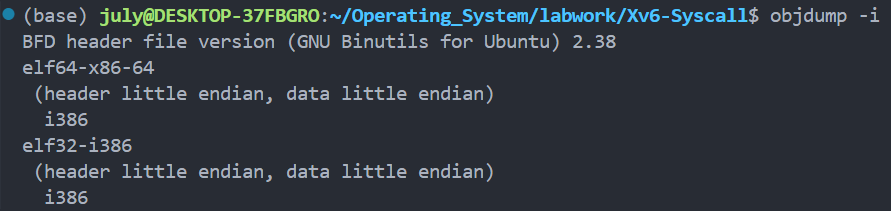
\includegraphics{E:/home/july/Operating_System/README.assets/SPYQufIx9qhJFmy.png}\\
如果第二行和我一样是\texttt{elf32-i386}就没问题了。

如果正常完成\hyperref[GNU]{GNU配置},\texttt{gcc}版本一定不会有问题的。

\begin{enumerate}
  \def\labelenumi{\arabic{enumi}.}
  \item
        编译xv6
\end{enumerate}

打开刚刚克隆的文件夹,例如\texttt{xv6-public},再运行\texttt{make}编译

\begin{Shaded}
  \begin{Highlighting}[]
    \BuiltInTok{cd}\NormalTok{ xv6{-}public}
    \FunctionTok{make}
  \end{Highlighting}
\end{Shaded}

\begin{quote}
  \texttt{make}包含在之前安装的\texttt{build-essential}包中,当目录下有\texttt{makefile}文件时会自动根据文件指示逐行编译(若指明的\texttt{.c}文件已经编译为\texttt{.o}则跳过,不会重复编译)。在后续我们添加系统调用的过程中,如果添加了新的\texttt{.c}文件,需要修改\texttt{makefile},加入新文件名,这样该文件可以在后续的\texttt{qemu}虚拟机窗口中作为可执行的命令被调用。
\end{quote}

\begin{enumerate}
  \def\labelenumi{\arabic{enumi}.}
  \item
        安装\texttt{qemu}虚拟机
\end{enumerate}

\begin{Shaded}
  \begin{Highlighting}[]
    \FunctionTok{sudo}\NormalTok{ apt{-}get install qemu{-}system}
  \end{Highlighting}
\end{Shaded}

(原先的命令已过时,\href{https://www.qemu.org/download/\#linux}{官网}已经更新了安装方式)

\begin{enumerate}
  \def\labelenumi{\arabic{enumi}.}
  \item
        用虚拟机启动Xv6
\end{enumerate}

\begin{Shaded}
  \begin{Highlighting}[]
    \FunctionTok{make}\NormalTok{ qemu}
  \end{Highlighting}
\end{Shaded}

\section{Guide to Lab works}\label{guide-to-lab-works}

\subsection{总体介绍------以Reverse为例}\label{ux603bux4f53ux4ecbux7ecd------ux4ee5reverseux4e3aux4f8b}

在VS
code中打开\texttt{\textasciitilde{}}目录,在\texttt{./projects/Reverse}下新建\texttt{reverse.c}文件。

\subsubsection{需求分析}\label{ux9700ux6c42ux5206ux6790}

\begin{enumerate}
  \def\labelenumi{\arabic{enumi}.}
  \item
        支持3种输入形式:

        \begin{itemize}
          \item
                \texttt{./reverse}
          \item
                \texttt{./reverse\ input.txt}
          \item
                \texttt{./reverse\ input.txt\ output.txt}
        \end{itemize}
  \item
        对于输入的数据(命令行/文件),\textbf{不能}假设\emph{句子长度}
        和\emph{句子个数}。
  \item
        处理以下4种错误:

        \begin{itemize}
          \item
                输入参数过多:\texttt{usage:\ reverse\ \textless{}input\textgreater{}\ \textless{}output\textgreater{}}
          \item
                文件无法打开:\texttt{reverse:\ cannot\ open\ file\ \textquotesingle{}\textless{}filename\textgreater{}\textquotesingle{}}(其中\texttt{\textless{}filename\textgreater{}}为打不开的文件名)
          \item
                输入相同文件:\texttt{reverse:\ input\ and\ output\ file\ must\ differ}(不能仅通过文件名判断)
          \item
                内存分配失败:\texttt{malloc\ failed}
        \end{itemize}
\end{enumerate}

\begin{quote}
  无论是哪一种错误,统一用\texttt{fprintf(stderr,\ "\textless{}error\ message\textgreater{}\textbackslash{}n");}输出错误并\texttt{exit(1);}返回状态码1。

  其中,stderr是一种特殊的输出流,与之类似的输出流是stdout,stdout类似c++中cout。

  返回的状态码正常为0,调用exit函数会立即终止并返回指定状态码。
\end{quote}

\subsubsection{功能实现}\label{ux529fux80fdux5b9eux73b0}

\begin{Shaded}
  \begin{Highlighting}[]
    \PreprocessorTok{\#include }\ImportTok{\textless{}stdio.h\textgreater{}}
    \PreprocessorTok{\#include }\ImportTok{\textless{}stdlib.h\textgreater{}}
    \PreprocessorTok{\#include }\ImportTok{\textless{}sys/stat.h\textgreater{}}
  \end{Highlighting}
\end{Shaded}

\begin{enumerate}
  \def\labelenumi{\arabic{enumi}.}
  \item
        处理错误``输入参数过多''
\end{enumerate}

\begin{Shaded}
  \begin{Highlighting}[]
    \CommentTok{// 如果用户运行时reverse参数过多,则打印usage: reverse \textless{}input\textgreater{} \textless{}output\textgreater{}并退出,返回码为 1}
    \ControlFlowTok{if} \OperatorTok{(}\NormalTok{argc }\OperatorTok{\textgreater{}} \DecValTok{3}\OperatorTok{)} \OperatorTok{\{}
    \NormalTok{    fprintf}\OperatorTok{(}\NormalTok{stderr}\OperatorTok{,} \StringTok{"usage: reverse \textless{}input\textgreater{} \textless{}output\textgreater{}}\SpecialCharTok{\textbackslash{}n}\StringTok{"}\OperatorTok{);}
    \NormalTok{    exit}\OperatorTok{(}\DecValTok{1}\OperatorTok{);}
    \OperatorTok{\}}
  \end{Highlighting}
\end{Shaded}

\begin{enumerate}
  \def\labelenumi{\arabic{enumi}.}
  \item
        处理错误``文件无法打开''
\end{enumerate}

\begin{Shaded}
  \begin{Highlighting}[]
    \CommentTok{// 输入流,文件或命令行输入(Ctrl+D结束输入)}
    \DataTypeTok{FILE} \OperatorTok{*}\NormalTok{input }\OperatorTok{=}\NormalTok{ stdin}\OperatorTok{;}

    \CommentTok{// 输出流,文件或命令行输出}
    \DataTypeTok{FILE} \OperatorTok{*}\NormalTok{output }\OperatorTok{=}\NormalTok{ stdout}\OperatorTok{;}

    \CommentTok{// 如果提供输入文件,打开输入文件}
    \ControlFlowTok{if} \OperatorTok{(}\NormalTok{argc }\OperatorTok{\textgreater{}=} \DecValTok{2}\OperatorTok{)} \OperatorTok{\{}
    \NormalTok{    input }\OperatorTok{=}\NormalTok{ fopen}\OperatorTok{(}\NormalTok{argv}\OperatorTok{[}\DecValTok{1}\OperatorTok{],} \StringTok{"r"}\OperatorTok{);}
    \ControlFlowTok{if} \OperatorTok{(}\NormalTok{input }\OperatorTok{==}\NormalTok{ NULL}\OperatorTok{)} \OperatorTok{\{}
    \NormalTok{        fprintf}\OperatorTok{(}\NormalTok{stderr}\OperatorTok{,} \StringTok{"reverse: cannot open file \textquotesingle{}}\SpecialCharTok{\%s}\StringTok{\textquotesingle{}}\SpecialCharTok{\textbackslash{}n}\StringTok{"}\OperatorTok{,}\NormalTok{ argv}\OperatorTok{[}\DecValTok{1}\OperatorTok{]);}
    \NormalTok{        exit}\OperatorTok{(}\DecValTok{1}\OperatorTok{);}
    \OperatorTok{\}}
    \OperatorTok{\}}

    \CommentTok{// 如果额外提供输出文件,尝试打开,并检查输入输出文件是否相同(用stat防止硬链接)}
    \ControlFlowTok{if} \OperatorTok{(}\NormalTok{argc }\OperatorTok{==} \DecValTok{3}\OperatorTok{)} \OperatorTok{\{}
    \NormalTok{    output }\OperatorTok{=}\NormalTok{ fopen}\OperatorTok{(}\NormalTok{argv}\OperatorTok{[}\DecValTok{2}\OperatorTok{],} \StringTok{"w"}\OperatorTok{);}
    \ControlFlowTok{if} \OperatorTok{(}\NormalTok{output }\OperatorTok{==}\NormalTok{ NULL}\OperatorTok{)} \OperatorTok{\{}
    \NormalTok{        fprintf}\OperatorTok{(}\NormalTok{stderr}\OperatorTok{,} \StringTok{"reverse: cannot open file \textquotesingle{}}\SpecialCharTok{\%s}\StringTok{\textquotesingle{}}\SpecialCharTok{\textbackslash{}n}\StringTok{"}\OperatorTok{,}\NormalTok{ argv}\OperatorTok{[}\DecValTok{2}\OperatorTok{]);}
    \NormalTok{        exit}\OperatorTok{(}\DecValTok{1}\OperatorTok{);}
    \OperatorTok{\}}
    \OperatorTok{\}}
  \end{Highlighting}
\end{Shaded}

\begin{enumerate}
  \def\labelenumi{\arabic{enumi}.}
  \item
        通过头文件\texttt{\textless{}sys/stat.h\textgreater{}}提供的stat函数处理错误``输入相同文件''
\end{enumerate}

\begin{Shaded}
  \begin{Highlighting}[]
    \KeywordTok{struct}\NormalTok{ stat stat1}\OperatorTok{,}\NormalTok{ stat2}\OperatorTok{;}
    \NormalTok{stat}\OperatorTok{(}\NormalTok{argv}\OperatorTok{[}\DecValTok{1}\OperatorTok{],} \OperatorTok{\&}\NormalTok{stat1}\OperatorTok{);}
    \NormalTok{stat}\OperatorTok{(}\NormalTok{argv}\OperatorTok{[}\DecValTok{2}\OperatorTok{],} \OperatorTok{\&}\NormalTok{stat2}\OperatorTok{);}
    \ControlFlowTok{if} \OperatorTok{(}\NormalTok{stat1}\OperatorTok{.}\NormalTok{st\_ino }\OperatorTok{==}\NormalTok{ stat2}\OperatorTok{.}\NormalTok{st\_ino}\OperatorTok{)} \OperatorTok{\{}
    \NormalTok{    fprintf}\OperatorTok{(}\NormalTok{stderr}\OperatorTok{,} \StringTok{"reverse: input and output file must differ}\SpecialCharTok{\textbackslash{}n}\StringTok{"}\OperatorTok{);}
    \NormalTok{    exit}\OperatorTok{(}\DecValTok{1}\OperatorTok{);}
    \OperatorTok{\}}
  \end{Highlighting}
\end{Shaded}

\begin{enumerate}
  \def\labelenumi{\arabic{enumi}.}
  \item
        分配初始内存,当容量不够时自动扩容,处理错误``内存分配失败''
\end{enumerate}

\begin{Shaded}
  \begin{Highlighting}[]
    \CommentTok{// 记录行数}
    \DataTypeTok{int}\NormalTok{ num\_lines }\OperatorTok{=} \DecValTok{0}\OperatorTok{;}

    \CommentTok{// 记录容量,初始为10}
    \DataTypeTok{int}\NormalTok{ capacity }\OperatorTok{=} \DecValTok{10}\OperatorTok{;}

    \CommentTok{// 用于存储行的数组}
    \DataTypeTok{char} \OperatorTok{**}\NormalTok{lines }\OperatorTok{=}\NormalTok{ malloc}\OperatorTok{(}\NormalTok{capacity }\OperatorTok{*} \KeywordTok{sizeof}\OperatorTok{(}\DataTypeTok{char} \OperatorTok{*));}
    \ControlFlowTok{if} \OperatorTok{(}\NormalTok{lines }\OperatorTok{==}\NormalTok{ NULL}\OperatorTok{)} \OperatorTok{\{}
    \NormalTok{    fprintf}\OperatorTok{(}\NormalTok{stderr}\OperatorTok{,} \StringTok{"malloc failed}\SpecialCharTok{\textbackslash{}n}\StringTok{"}\OperatorTok{);}
    \NormalTok{    exit}\OperatorTok{(}\DecValTok{1}\OperatorTok{);}
    \OperatorTok{\}}

    \DataTypeTok{size\_t}\NormalTok{ len }\OperatorTok{=} \DecValTok{0}\OperatorTok{;}
    \ControlFlowTok{while} \OperatorTok{(}\DecValTok{1}\OperatorTok{)} \OperatorTok{\{}
    \ControlFlowTok{if} \OperatorTok{(}\NormalTok{num\_lines }\OperatorTok{==}\NormalTok{ capacity}\OperatorTok{)} \OperatorTok{\{}
    \NormalTok{        capacity }\OperatorTok{*=} \DecValTok{2}\OperatorTok{;}
    \NormalTok{        lines }\OperatorTok{=}\NormalTok{ realloc}\OperatorTok{(}\NormalTok{lines}\OperatorTok{,}\NormalTok{ capacity }\OperatorTok{*} \KeywordTok{sizeof}\OperatorTok{(}\DataTypeTok{char} \OperatorTok{*));}
    \ControlFlowTok{if} \OperatorTok{(}\NormalTok{lines }\OperatorTok{==}\NormalTok{ NULL}\OperatorTok{)} \OperatorTok{\{}
    \NormalTok{            fprintf}\OperatorTok{(}\NormalTok{stderr}\OperatorTok{,} \StringTok{"malloc failed}\SpecialCharTok{\textbackslash{}n}\StringTok{"}\OperatorTok{);}
    \NormalTok{            exit}\OperatorTok{(}\DecValTok{1}\OperatorTok{);}
    \OperatorTok{\}}
    \OperatorTok{\}}
    \ControlFlowTok{if} \OperatorTok{(}\NormalTok{getline}\OperatorTok{(\&}\NormalTok{lines}\OperatorTok{[}\NormalTok{num\_lines}\OperatorTok{],} \OperatorTok{\&}\NormalTok{len}\OperatorTok{,}\NormalTok{ input}\OperatorTok{)} \OperatorTok{==} \OperatorTok{{-}}\DecValTok{1}\OperatorTok{)}
    \ControlFlowTok{break}\OperatorTok{;}
    \NormalTok{    num\_lines}\OperatorTok{++;}
    \OperatorTok{\}}
  \end{Highlighting}
\end{Shaded}

\begin{quote}
  \texttt{getline}函数在\texttt{len}设置为0时,会自动扩充输入缓冲区并更新\texttt{len}参数。

  如果想通过终端测试零参数下的效果,可通过\texttt{Ctrl+D}终止输入流,此时\texttt{getline}函数会返回-1。
\end{quote}

\begin{enumerate}
  \def\labelenumi{\arabic{enumi}.}
  \item
        将获取的所有句子逆序放入输出流,释放内存并关闭文件
\end{enumerate}

\begin{Shaded}
  \begin{Highlighting}[]
    \ControlFlowTok{for} \OperatorTok{(}\DataTypeTok{int}\NormalTok{ i }\OperatorTok{=}\NormalTok{ num\_lines }\OperatorTok{{-}} \DecValTok{1}\OperatorTok{;}\NormalTok{ i }\OperatorTok{\textgreater{}=} \DecValTok{0}\OperatorTok{;}\NormalTok{ i}\OperatorTok{{-}{-})} \OperatorTok{\{}
    \NormalTok{    fprintf}\OperatorTok{(}\NormalTok{output}\OperatorTok{,} \StringTok{"}\SpecialCharTok{\%s}\StringTok{"}\OperatorTok{,}\NormalTok{ lines}\OperatorTok{[}\NormalTok{i}\OperatorTok{]);}
    \NormalTok{    free}\OperatorTok{(}\NormalTok{lines}\OperatorTok{[}\NormalTok{i}\OperatorTok{]);}
    \OperatorTok{\}}

    \NormalTok{free}\OperatorTok{(}\NormalTok{lines}\OperatorTok{);}

    \ControlFlowTok{if} \OperatorTok{(}\NormalTok{input }\OperatorTok{!=}\NormalTok{ stdin}\OperatorTok{)}
    \NormalTok{    fclose}\OperatorTok{(}\NormalTok{input}\OperatorTok{);}
    \ControlFlowTok{if} \OperatorTok{(}\NormalTok{output }\OperatorTok{!=}\NormalTok{ stdout}\OperatorTok{)}
    \NormalTok{    fclose}\OperatorTok{(}\NormalTok{output}\OperatorTok{);}
  \end{Highlighting}
\end{Shaded}

\begin{quote}
  注意,与C++不同,C语言中用malloc分配的内存一定要主动调用free函数进行内存释放,文件需要主动关闭,这是比较好的代码习惯。
\end{quote}

\subsubsection{编译文件并测试功能}\label{ux7f16ux8bd1ux6587ux4ef6ux5e76ux6d4bux8bd5ux529fux80fd}

\begin{enumerate}
  \def\labelenumi{\arabic{enumi}.}
  \item
        选中文件,右键``在集成终端中打开''
  \item
        输入\texttt{gcc\ -o\ reverse\ reverse.c\ -Wall}进行编译
  \item
        输入\texttt{sudo\ chmod\ 777\ test-reverse.sh}对当前测试脚本的权限进行修改

        (你可能还需要输入\texttt{sudo\ chmod\ 777\ ../tester/*}将其他测试脚本的权限设为最高)
  \item
        输入\texttt{./test-reverse.sh}进行测试。

        如果一切顺利的话,你会看到以下结果

        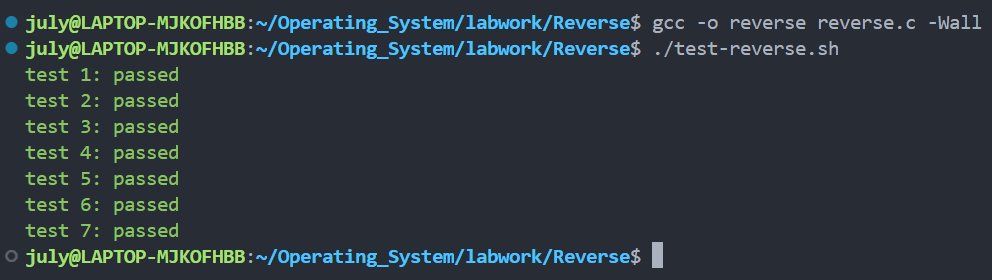
\includegraphics{E:/home/july/Operating_System/README.assets/XQ1hLsDiR2Pnrwz.png}
\end{enumerate}

\subsection{Kernel Hacking介绍}\label{kernel-hackingux4ecbux7ecd}

\begin{enumerate}
  \def\labelenumi{\arabic{enumi}.}
  \item
        开始实验
\end{enumerate}

在文件夹\texttt{Xv6-Syscal}中打开终端。

首先,手动把刚刚的文件夹\texttt{xv6-public}改名为\texttt{src},并修改测试文件权限。

(假设\texttt{../test}文件夹中的脚本均已设为最高权限)

\begin{Shaded}
  \begin{Highlighting}[]
    \FunctionTok{sudo}\NormalTok{ chmod 777 test{-}getreadcount.sh}
    \ExtensionTok{./test{-}getreadcount.sh}
  \end{Highlighting}
\end{Shaded}

如果不出意外的话,程序会开始运行,并抛出一个错误:

\includegraphics{E:/home/july/Operating_System/README.assets/p7QnysPA3mNTGdB.png}

这是正常的,因为\texttt{getreadcount()}函数需要我们自己实现。

这一部分实验建议参考Xv6官方的\href{https://github.com/remzi-arpacidusseau/ostep-projects/tree/master/initial-xv6}{介绍},相比于现在的介绍多了一些Tips和教学视频。

\subsubsection{功能分析}\label{ux529fux80fdux5206ux6790}

看一下test\_1.c代码:

\begin{Shaded}
  \begin{Highlighting}[]
    \PreprocessorTok{\#include }\ImportTok{"types.h"}
    \PreprocessorTok{\#include }\ImportTok{"stat.h"}
    \PreprocessorTok{\#include }\ImportTok{"user.h"}

    \DataTypeTok{int}\NormalTok{ main}\OperatorTok{(}\DataTypeTok{int}\NormalTok{ argc}\OperatorTok{,} \DataTypeTok{char} \OperatorTok{*}\NormalTok{argv}\OperatorTok{[])}
    \OperatorTok{\{}
    \DataTypeTok{int}\NormalTok{ x1 }\OperatorTok{=}\NormalTok{ getreadcount}\OperatorTok{();}
    \DataTypeTok{int}\NormalTok{ x2 }\OperatorTok{=}\NormalTok{ getreadcount}\OperatorTok{();}
    \DataTypeTok{char}\NormalTok{ buf}\OperatorTok{[}\DecValTok{100}\OperatorTok{];}
    \OperatorTok{(}\DataTypeTok{void}\OperatorTok{)}\NormalTok{read}\OperatorTok{(}\DecValTok{4}\OperatorTok{,}\NormalTok{ buf}\OperatorTok{,} \DecValTok{1}\OperatorTok{);}
    \DataTypeTok{int}\NormalTok{ x3 }\OperatorTok{=}\NormalTok{ getreadcount}\OperatorTok{();}
    \DataTypeTok{int}\NormalTok{ i}\OperatorTok{;}
    \ControlFlowTok{for} \OperatorTok{(}\NormalTok{i }\OperatorTok{=} \DecValTok{0}\OperatorTok{;}\NormalTok{ i }\OperatorTok{\textless{}} \DecValTok{1000}\OperatorTok{;}\NormalTok{ i}\OperatorTok{++)}
    \OperatorTok{\{}
    \OperatorTok{(}\DataTypeTok{void}\OperatorTok{)}\NormalTok{read}\OperatorTok{(}\DecValTok{4}\OperatorTok{,}\NormalTok{ buf}\OperatorTok{,} \DecValTok{1}\OperatorTok{);}
    \OperatorTok{\}}
    \DataTypeTok{int}\NormalTok{ x4 }\OperatorTok{=}\NormalTok{ getreadcount}\OperatorTok{();}
    \NormalTok{  printf}\OperatorTok{(}\DecValTok{1}\OperatorTok{,} \StringTok{"XV6\_TEST\_OUTPUT }\SpecialCharTok{\%d}\StringTok{ }\SpecialCharTok{\%d}\StringTok{ }\SpecialCharTok{\%d\textbackslash{}n}\StringTok{"}\OperatorTok{,}\NormalTok{ x2 }\OperatorTok{{-}}\NormalTok{ x1}\OperatorTok{,}\NormalTok{ x3 }\OperatorTok{{-}}\NormalTok{ x2}\OperatorTok{,}\NormalTok{ x4 }\OperatorTok{{-}}\NormalTok{ x3}\OperatorTok{);}
    \NormalTok{  exit}\OperatorTok{();}
    \OperatorTok{\}}
  \end{Highlighting}
\end{Shaded}

可以看到导入了3个头文件,其中\texttt{types.h}提供了一些基本类型的定义,\texttt{stat.h}提供了一个结构体\texttt{stat}的定义:

\begin{Shaded}
  \begin{Highlighting}[]
    \PreprocessorTok{\#define T\_DIR  }\DecValTok{1}\PreprocessorTok{   }\CommentTok{// Directory}
    \PreprocessorTok{\#define T\_FILE }\DecValTok{2}\PreprocessorTok{   }\CommentTok{// File}
    \PreprocessorTok{\#define T\_DEV  }\DecValTok{3}\PreprocessorTok{   }\CommentTok{// Device}

    \KeywordTok{struct}\NormalTok{ stat }\OperatorTok{\{}
    \DataTypeTok{short}\NormalTok{ type}\OperatorTok{;}  \CommentTok{// Type of file}
    \DataTypeTok{int}\NormalTok{ dev}\OperatorTok{;}     \CommentTok{// File system\textquotesingle{}s disk device}
    \NormalTok{  uint ino}\OperatorTok{;}    \CommentTok{// Inode number}
    \DataTypeTok{short}\NormalTok{ nlink}\OperatorTok{;} \CommentTok{// Number of links to file}
    \NormalTok{  uint size}\OperatorTok{;}   \CommentTok{// Size of file in bytes}
    \OperatorTok{\};}
  \end{Highlighting}
\end{Shaded}

这里,首先把所有文件分为了\texttt{目录},\texttt{文件}和\texttt{设备}(Unix系统中,一般把设备看作特殊的文件对象),这里所谓的\texttt{short\ type}就是以上3种类型之一。接下来,定义了\texttt{dev}设备编号,\texttt{ino}文件\texttt{incde}号,别名个数和文件大小。

系统调用至少需要修改以下文件:

\begin{longtable}[]{@{}ll@{}}
  \toprule\noalign{}
  文件        & 简介                                         \\
  \midrule\noalign{}
  \endhead
  \bottomrule\noalign{}
  \endlastfoot
  usys.S    & 提供系统调用入口                                   \\
  syscall.h & 定义系统调用编号SYS\_\textless{}name\textgreater{} \\
            &                                            \\
            &                                            \\
\end{longtable}

\end{document}
